\documentclass{standalone}

\usepackage{tikz}

\begin{document}
  %noformat{
  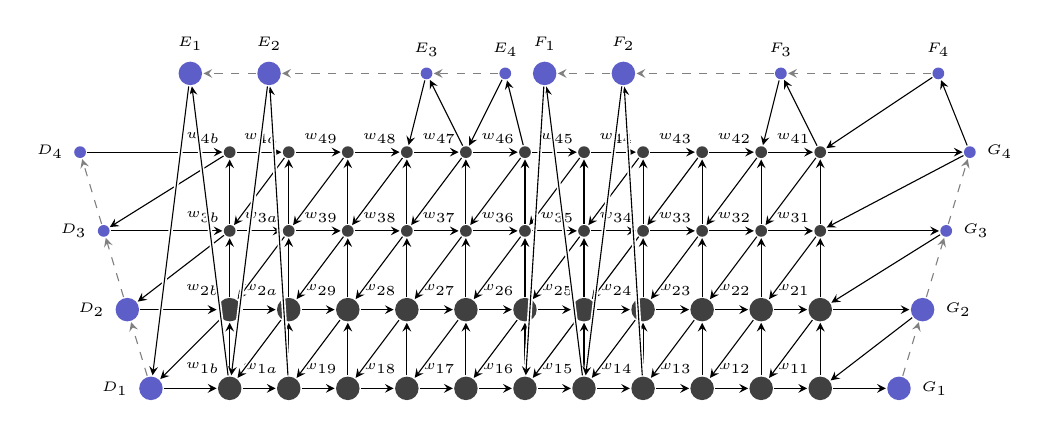
\begin{tikzpicture}
    \tikzstyle{v1} = [circle, outer xsep=0.5pt, fill, inner sep=1.5pt]
    \tikzstyle{v2} = [circle, outer xsep=0.5pt, fill, inner sep=3.0pt]
    \tikzstyle{unf} = [color=darkgray]
    \tikzstyle{frz} = [color=blue!60!darkgray!70]
    \tikzstyle{e} = [->, >={stealth}, preaction={draw=white, -, ultra thick}]
    \tikzstyle{h} = [dashed, color=gray, ->, >={stealth}]

    \tikzset{font=\tiny}
    
    \foreach \l/\p/\x in { b/11/1.0, a/10/1.75, 9/9/2.5, 8/8/3.25, 7/7/4.0, 6/6/4.75, 5/5/5.5, 4/4/6.25, 3/3/7.0, 2/2/7.75, 1/1/8.5 } {
        \node[v2,label={[label distance=-3pt]95:{$w_{1\l}$}}, unf] (v1\p) at (\x,0) {};
        \node[v2,label={[label distance=-3pt]95:{$w_{2\l}$}}, unf] (v2\p) at (\x,1) {};
        \node[v1,label={[label distance=-3pt]95:{$w_{3\l}$}}, unf] (v3\p) at (\x,2) {};
        \node[v1,label={[label distance=-3pt]95:{$w_{4\l}$}}, unf] (v4\p) at (\x,3) {};
    }

    \node[v2,label=180:{$D_1$}, frz] (D1) at (-0.0,0) {};
    \node[v2,label=180:{$D_2$}, frz] (D2) at (-0.3,1) {};
    \node[v1,label=180:{$D_3$}, frz] (D3) at (-0.6,2) {};
    \node[v1,label=180:{$D_4$}, frz] (D4) at (-0.9,3) {};

    \node[v2,label=0:{$G_{1}$}, frz] (G1) at ( 9.5,0) {};
    \node[v2,label=0:{$G_{2}$}, frz] (G2) at ( 9.8,1) {};
    \node[v1,label=0:{$G_{3}$}, frz] (G3) at (10.1,2) {};
    \node[v1,label=0:{$G_{4}$}, frz] (G4) at (10.4,3) {};

    \node[v1,label=90:{$F_{4}$}, frz] (F4) at (10,4) {};
    \node[v1,label=90:{$F_{3}$}, frz] (F3) at ( 8,4) {};
    \node[v2,label=90:{$F_{2}$}, frz] (F2) at ( 6,4) {};
    \node[v2,label=90:{$F_{1}$}, frz] (F1) at ( 5,4) {};

    \node[v1,label=90:{$E_{4}$}, frz] (E4) at ( 4.5,4) {};
    \node[v1,label=90:{$E_{3}$}, frz] (E3) at ( 3.5,4) {};
    \node[v2,label=90:{$E_{2}$}, frz] (E2) at ( 1.5,4) {};
    \node[v2,label=90:{$E_{1}$}, frz] (E1) at ( 0.5,4) {};

    \foreach \p in {G, D} {
      \draw[h] (\p1) -- (\p2);
      \draw[h] (\p2) -- (\p3);
      \draw[h] (\p3) -- (\p4);
    }
    \foreach \p in {E, F} {
      \draw[h] (\p2) -- (\p1);
      \draw[h] (\p3) -- (\p2);
      \draw[h] (\p4) -- (\p3);
    }
    \foreach \p in {1, 2, ..., 11} {
      \draw[e] (v1\p) -- (v2\p);
      \draw[e] (v2\p) -- (v3\p);
      \draw[e] (v3\p) -- (v4\p);
    }

    \foreach \p in {1, 2, ..., 10} {
      \pgfmathtruncatemacro\q{\p + 1}
      \draw[e] (v1\q) -- (v1\p);
      \draw[e] (v2\q) -- (v2\p);
      \draw[e] (v3\q) -- (v3\p);
      \draw[e] (v4\q) -- (v4\p);

      \draw[e] (v2\p) -- (v1\q);
      \draw[e] (v3\p) -- (v2\q);
      \draw[e] (v4\p) -- (v3\q);
    }

    \draw[e] (v11) -- (G1);
    \draw[e]  (G2) -- (v11);
    \draw[e] (v21) -- (G2);
    \draw[e]  (G3) -- (v21);
    \draw[e] (v31) -- (G3);
    \draw[e]  (G4) -- (v31);
    \draw[e] (v41) -- (G4);

    \draw[e]   (D1) -- (v111);
    \draw[e] (v211) --   (D1);
    \draw[e]   (D2) -- (v211);
    \draw[e] (v311) --   (D2);
    \draw[e]   (D3) -- (v311);
    \draw[e] (v411) --   (D3);
    \draw[e]   (D4) -- (v411);

    \foreach \from/\to in {v111/E1, E1/D1, v110/E2, E2/v111, v47/E3, E3/v48, v46/E4, E4/v47} {
      \draw[e] (\from) -- (\to);
    }

    \foreach \from/\to in {v15/F1, F1/v16, v14/F2, F2/v15, v41/F3, F3/v42, G4/F4, F4/v41} {
      \draw[e] (\from) -- (\to);
    }

  \end{tikzpicture}
  %}noformat
\end{document}
